\chapter{Structural Properties of Semiconductors}

\section{Crystal Growth}
\subsection{Bulk Crystal Growth}
Semiconductor technology depends critycally upon the availability  of high quality substrates with as large a diameter as possible. Bulk crystal growth techniques are used mainly
to produce substrates on which devices are eventually fabricated. While for some semiconductors like Si and GaAs the bulk crystal growth techniques are higly matured.
For the growth of boules from which substrates are obtained, one start out wiht a purified from of the elements that are to make up the crystal. \\
One of the most important technique that is used is the Czochralski method, which is used to grow single crystal silicon boules. The process involves melting high purity silicon in a crucible and then dipping a seed crystal into the melt. The seed crystal is slowly pulled upwards while rotating, allowing the silicon to crystallize onto the seed.
The CZ techinique is widely employed for Si, GaAs and InP.\\\\
A second bulk crystal growth technique involves a charge of material loaded in quartz container. The charge may be composed of either high quality polycrystalline material or carefully measured quantities of elements which make up a compound
crystal. The containser called a "boat" is heated till the charge melts and wets the seed crystal.\\
The seed is then used to crystallize the melt by slowly loweing the boat temperature starting from the seed end.\\
The easiest approach for the boat technique is to use a horizontal boat. However, the shape of the boule that is produced has a D-shaped form.
\begin{center}
	\begin{minipage}{0.8\textwidth}
		\centering
		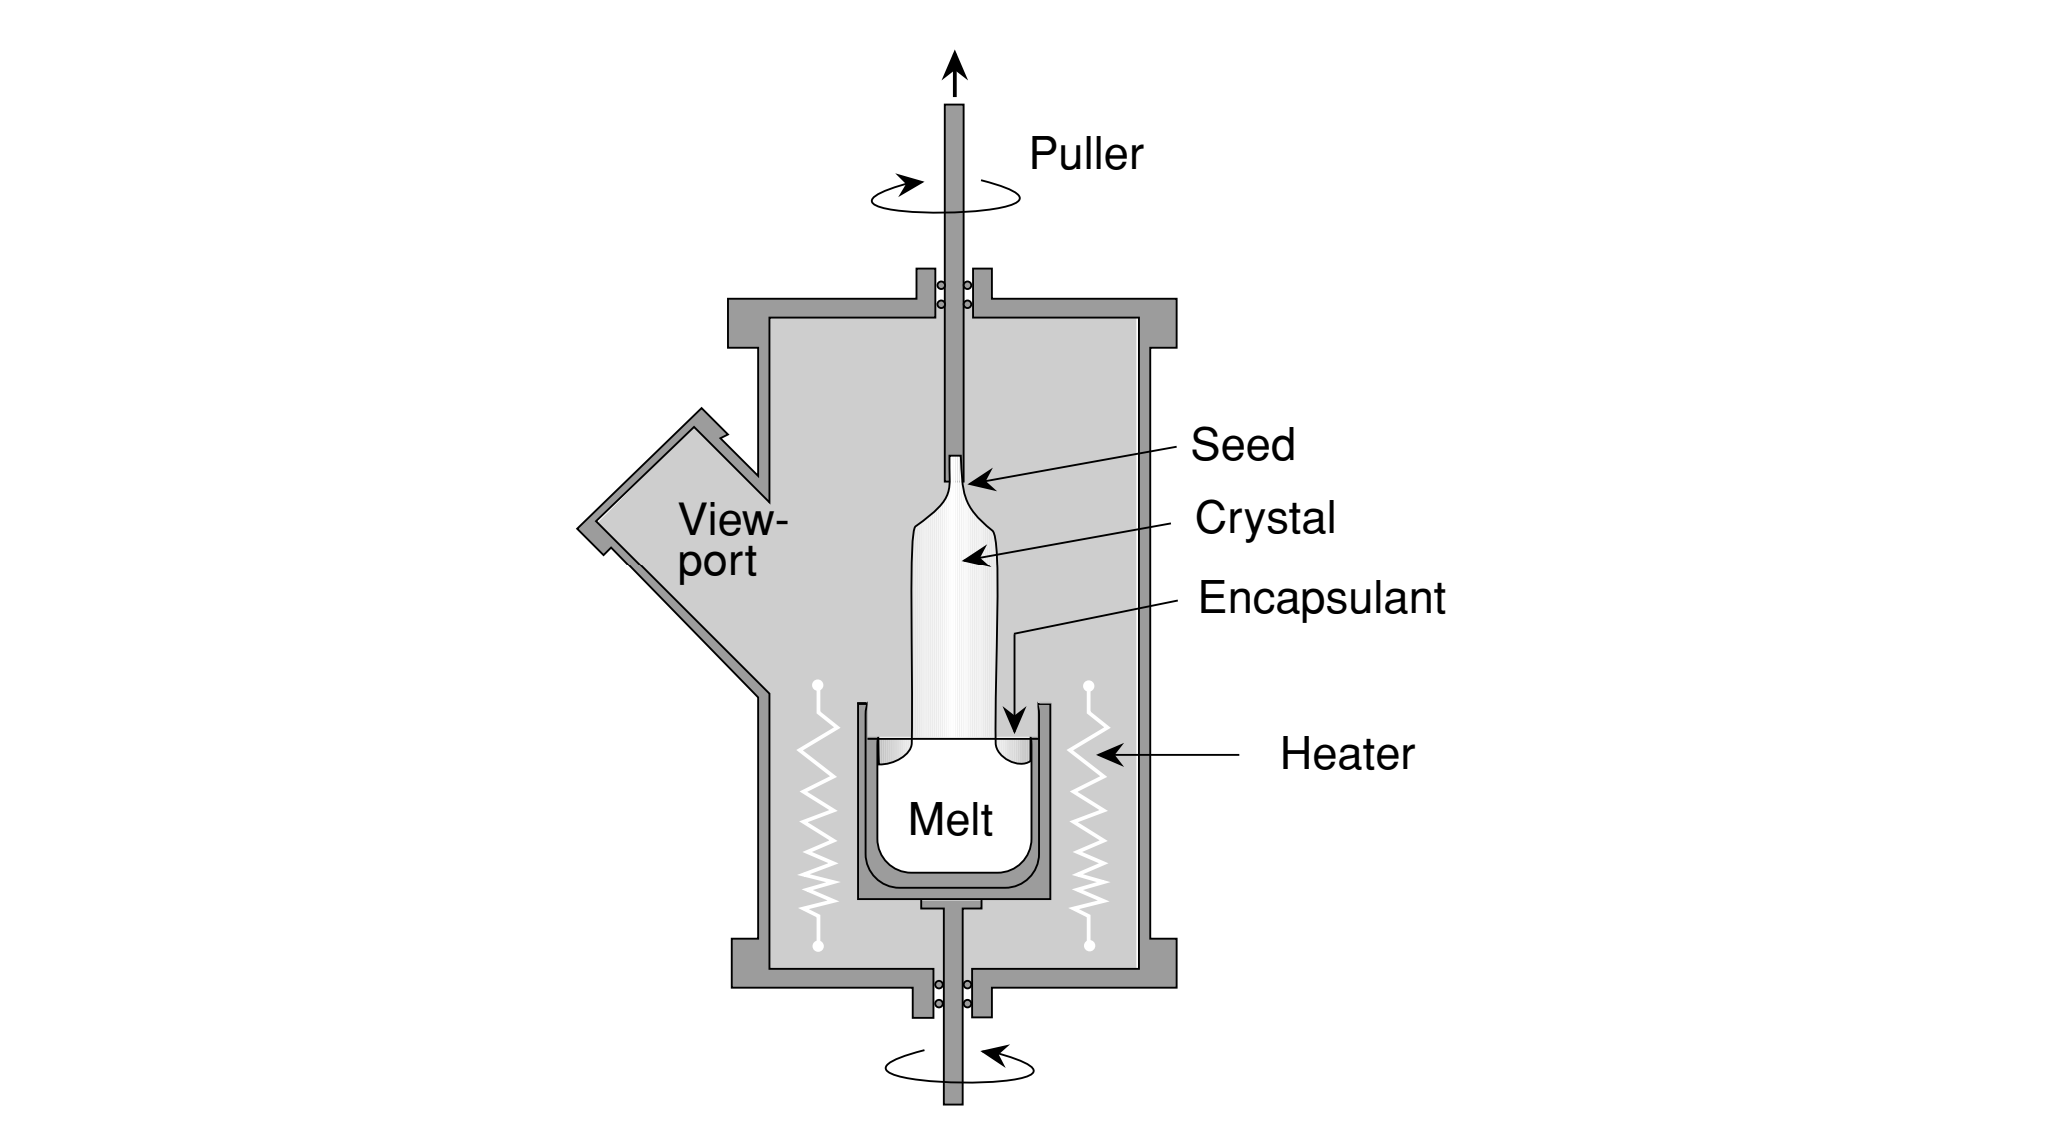
\includegraphics[width=\textwidth]{img/Czochralski.png}
		\\[0.5em]
		\refstepcounter{figure}
		\textbf{Figure~\thefigure.} Schematic of the Czochralski (CZ) method for growing single crystal silicon boules.
		\label{fig:CZ}
	\end{minipage}
\end{center}


\subsection{MBE: Molecular Beam Epitaxy}
MBE is capable of controlling deposition of submonolayer coverage on a substrate and has become one of the most important epitaxial techniques. Almost every semiconductor
has been grown by this technique. MBE is a high vacuum technique in which crucibles containing a variety of elemental charges are placed in the growth chamber.\\
The elements contained in the crucibles make up the components of the crystal to be grown as well as the dopants that may be used. When a crucible is heated, atoms or molecules of the charge are evaporated and these travel in straight lines to impinge on a heated substrate. \\
The growth rate in MBE is $\sim 1.0$ monolayer per second and this slow rate, coupled with shutters placed in front of the crucibles, allows one to switch the composition of the growing crystal with monolayer control. Since no chemical reactions occur in MBE,
the growth is the simplest of all epitaxial techniques and is quite controllable. However, since the growth involves high vacuum, leaks can be a major problem.
The low background pressure in MBE allows one to use electron beams to monitor the growing crystal.
\begin{center}
	\begin{minipage}{0.63\textwidth}
		\centering
		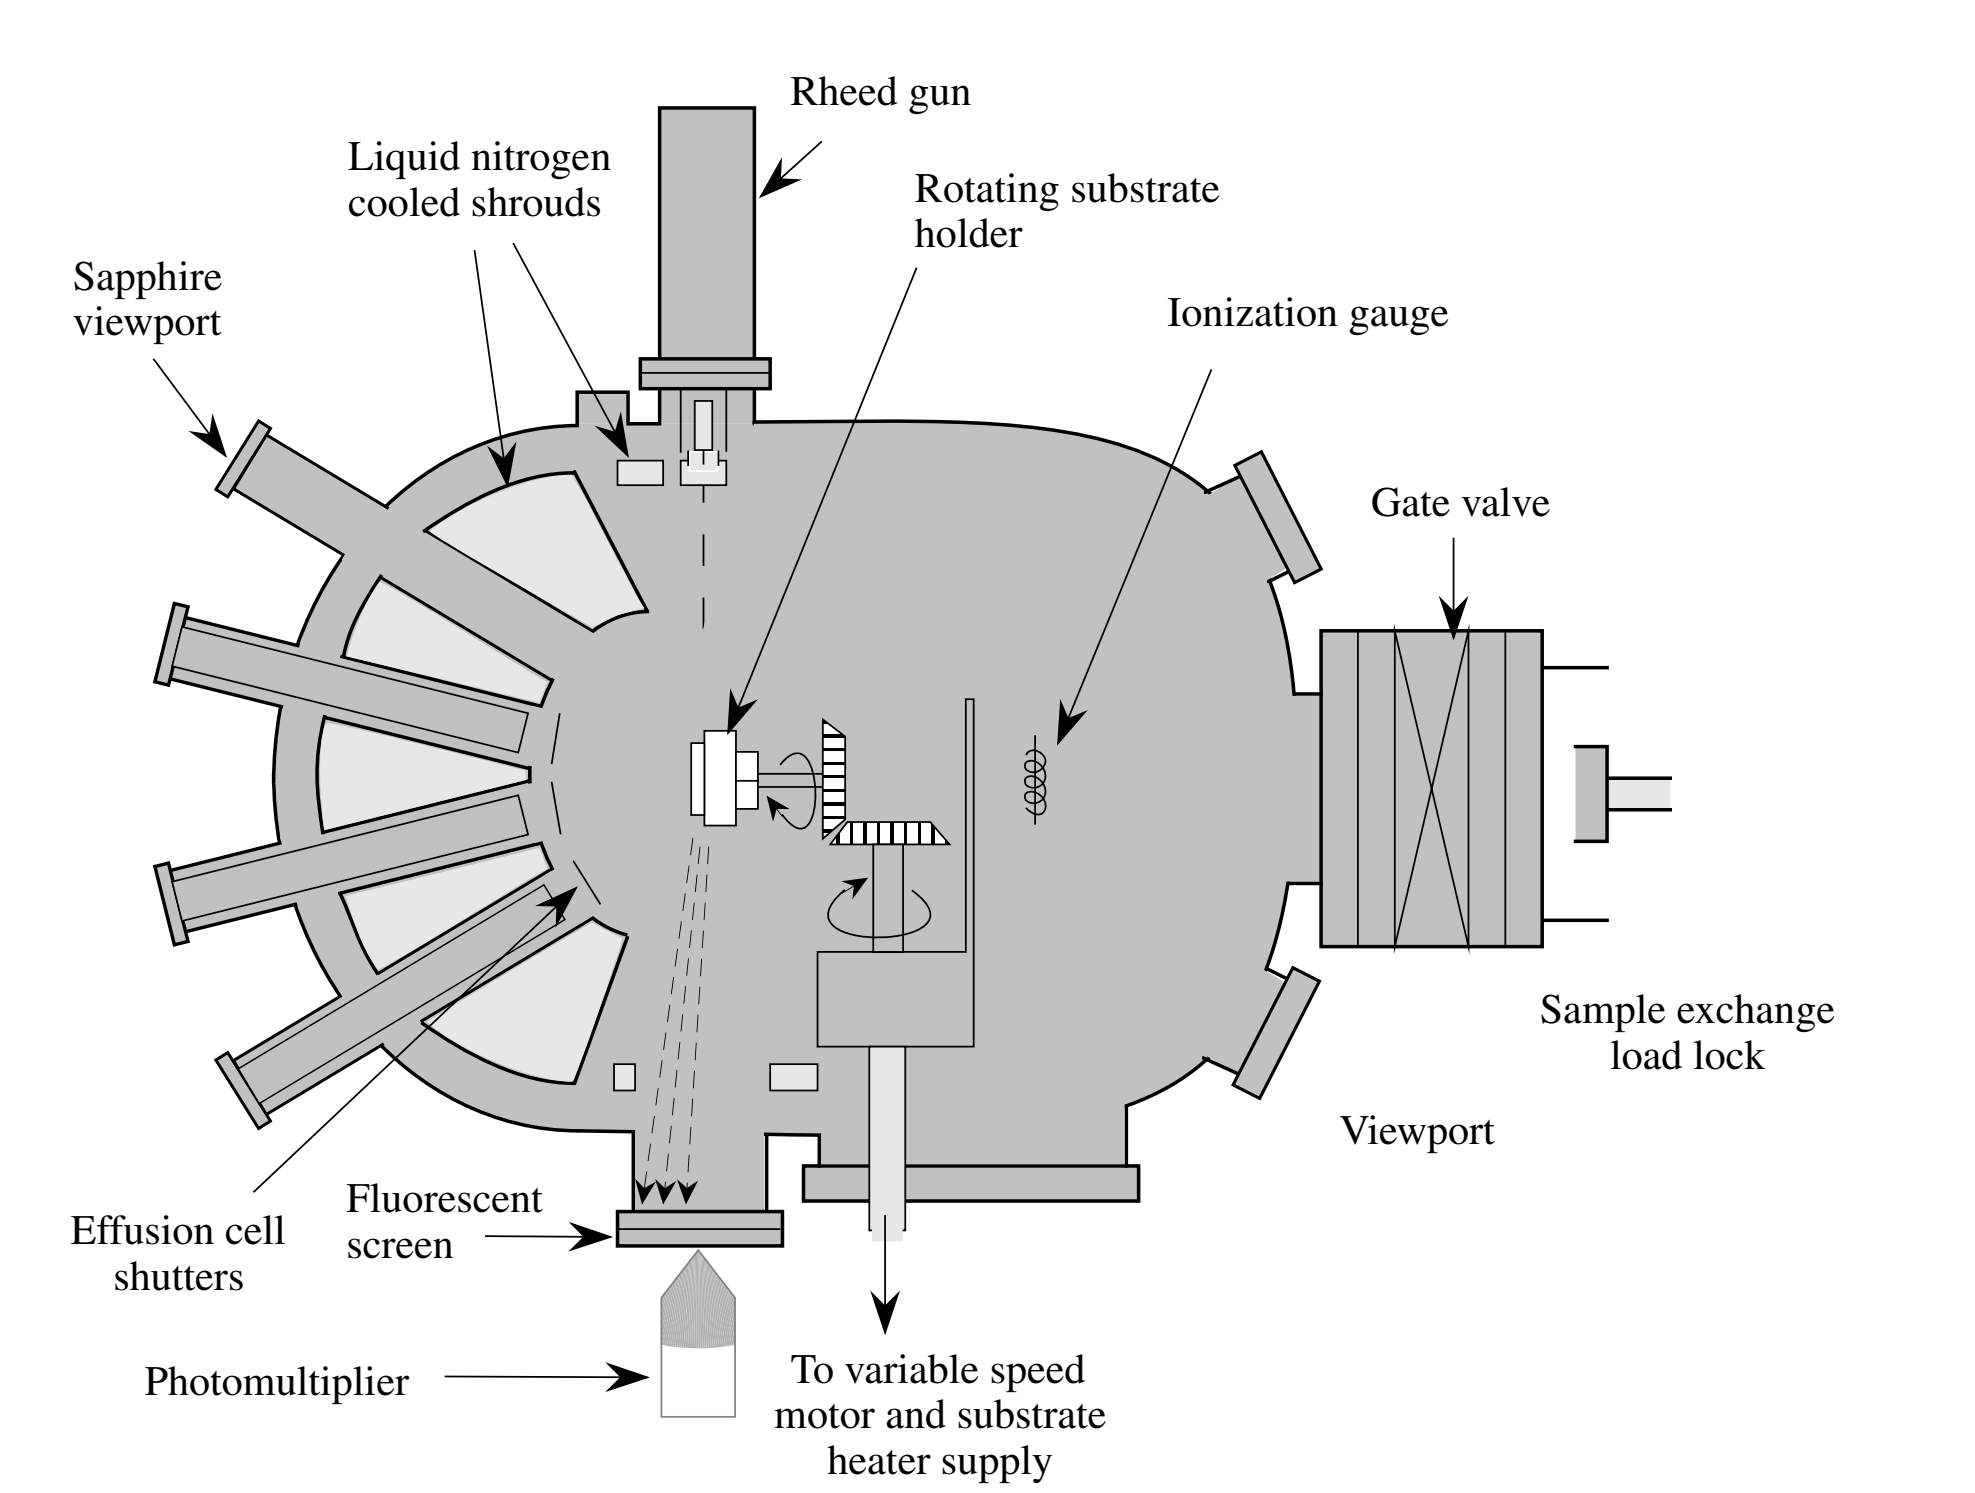
\includegraphics[width=\textwidth]{img/MBE.png}
		\\[0.5em]
		\refstepcounter{figure}
		\textbf{Figure~\thefigure.} Schematic of a molecular beam epitaxy (MBE) system.
		\label{fig:MBE}
	\end{minipage}
\end{center}

\section{Crystal Structure}
Crystals are composed of identical fundamental units, which can be individual atoms or clusters of atoms. In naturally occurring crystals, the crystalline symmetry is inherent and determined by natural processes. However, recent developments in crystal growth techniques now enable scientists to create artificial crystals with altered crystalline structures.\\
To define a crystal structure, we use two key concepts. First, the lattice is an abstract, periodically arranged set of points in space, where every point has an identical environment. Second, a basis, which is a group of atoms, is attached to each of these lattice points, creating the full crystal structure.\\
An important property of lattice is the ability to define three vectors $\mathbf{a}_1$, $\mathbf{a}_2$, and $\mathbf{a}_3$, such that any lattice point $\mathbf{R'}$ can be expressed as:
\begin{equation*}
	\mathbf{R'} = \mathbf{R} + m_1 \mathbf{a}_1 + m_2 \mathbf{a}_2 + m_3 \mathbf{a}_3
\end{equation*}
where $\mathbf{R}$ is a lattice point, and $m_1$, $m_2$, and $m_3$ are integers. Such a lattice is called \textbf{Bravais lattice}. The vectors $\mathbf{a}_1$, $\mathbf{a}_2$, and $\mathbf{a}_3$ are called the lattice vectors, and they define the unit cell of the crystal. The unit cell is the smallest repeating unit that can be used to construct the entire crystal structure by translation along the lattice vectors.\\
%Create a box with wtitten lattice + basis = crysal structure
\begin{center}
	\begin{minipage}{0.5\textwidth}
		\centering
		\fbox{
			\begin{minipage}{0.9\textwidth}
				\centering
				\textbf{Lattice + Basis = Crystal Structure}
			\end{minipage}
		}
	\end{minipage}
\end{center}

The translation vectors $\mathbf{a}_1$, $\mathbf{a}_2$, and $\mathbf{a}_3$ are called primitive if the volume of the celle is formed by them is the smallest possible. There is no unique way to choose the primitive vectors. One choice is to pick:
\begin{itemize}
	\item $\mathbf{a}_1$ to be the shortest period in the lattice;
	\item $\mathbf{a}_2$ to be the shortest period not parallel to $\mathbf{a}_1$;
	\item $\mathbf{a}_3$ to be the shortest period not coplanar to $\mathbf{a}_1$ and $\mathbf{a}_2$.
\end{itemize}
The volume cell enclosed by the primitive vectors is called the primitive cell, and it is the smallest volume that can be used to construct the entire crystal structure by translation along the lattice vectors.\\
Due to the periodic nature of a lattice, it's helpful to establish the structure's symmetry. This symmetry is characterized by a group of point group operations, which are transformations performed around a specific point. These operations include \textbf{rotation, reflection, and inversion.}
The symmetry of a crystal significantly influences its electronic properties.

\subsection{Lattice Types}
The different types of lattice structures found in nature are characterized by their \textbf{symmetry groups}, with \textbf{rotation} being a crucial one. Lattices can exhibit rotational symmetries of $2\pi$, $\frac{2\pi}{2}$, $\frac{2\pi}{3}$, $\frac{2\pi}{4}$, and $\frac{2\pi}{6}$. These are commonly denoted as 1, 2, 3, 4, and 6, respectively. Other rotation axes, such as $\frac{2\pi}{5}$ or $\frac{2\pi}{7}$, are not permitted because such structures cannot completely fill an infinite space.\\
In three dimensions, there are 14 distinct types of lattices. These lattice classes are defined by the relationships between their \textbf{primitive vectors} $\mathbf{a}_1$, $\mathbf{a}_2$, and $\mathbf{a}_3$, as well as the \textbf{angles} $\alpha$, $\beta$, and $\gamma$ between them. The most general lattice is \textbf{triclinic} (where $\alpha \neq \beta \neq \gamma$ and $\mathbf{a}_1 \neq \mathbf{a}_2 \neq \mathbf{a}_3$), and there are 13 additional special lattice types.\\
We will focus on the \textbf{cubic lattice}, which is the structure adopted by all semiconductors. There are three types of cubic lattices: \textbf{simple cubic}, \textbf{body-centered cubic}, and \textbf{face-centered cubic}.\\

\begin{center}
	\begin{minipage}{0.4\textwidth}
		\centering
		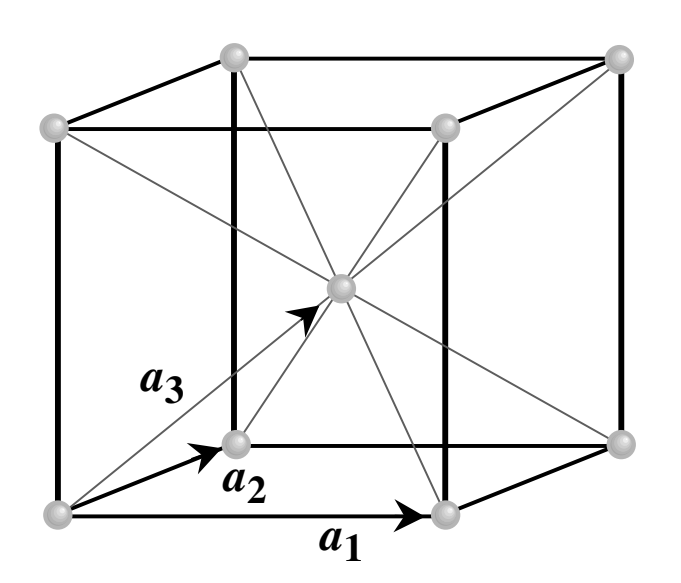
\includegraphics[width=\textwidth]{img/cubic_lattice.png}
		\\[0.5em]
		\refstepcounter{figure}
		\textbf{Figure~\thefigure.} Schematic of the cubic lattice structure.
		\label{fig:cubic_lattice}
	\end{minipage}
\end{center}

\subsubsection{Simple Cubic}
The simple cubic lattice is generated by the primitive vectors
\begin{align*}
	a\mathbf{x}, a\mathbf{y}, a\mathbf{z}
\end{align*}
where the $\mathbf{x}, \mathbf{y}, \mathbf{z}$ are unit vectors.

\subsubsection{Body-Centered Cubic}
The bcc lattice can be generated from the simple cubic structure by placing a lattice point at the center of the cube. If $\mathbf{\hat{x}}$, $\mathbf{\hat{y}}$, and $\mathbf{\hat{z}}$ are three orthogonal unit vectors, then a set of primitive vectors for the body-centered cubic lattice could be
\begin{align*}
	\mathbf{a_1} = a\mathbf{\hat{x}}, \quad \mathbf{a_2} = a\mathbf{\hat{y}}, \quad \mathbf{a_3} = a\mathbf{\hat{z}}
\end{align*}
A more symmetric set for the bcc lattice is
\begin{align*}
	\mathbf{a_1} & = \frac{a}{2}(\mathbf{\hat{y}} + \mathbf{\hat{z}} - \mathbf{\hat{x}}), \\
	\mathbf{a_2} & = \frac{a}{2}(\mathbf{\hat{x}} + \mathbf{\hat{z}} - \mathbf{\hat{y}}), \\
	\mathbf{a_3} & = \frac{a}{2}(\mathbf{\hat{x}} + \mathbf{\hat{y}} - \mathbf{\hat{z}})
\end{align*}


\subsubsection{Face-Centered Cubic}

\begin{center}
	\begin{minipage}{0.5\textwidth}
		\centering
		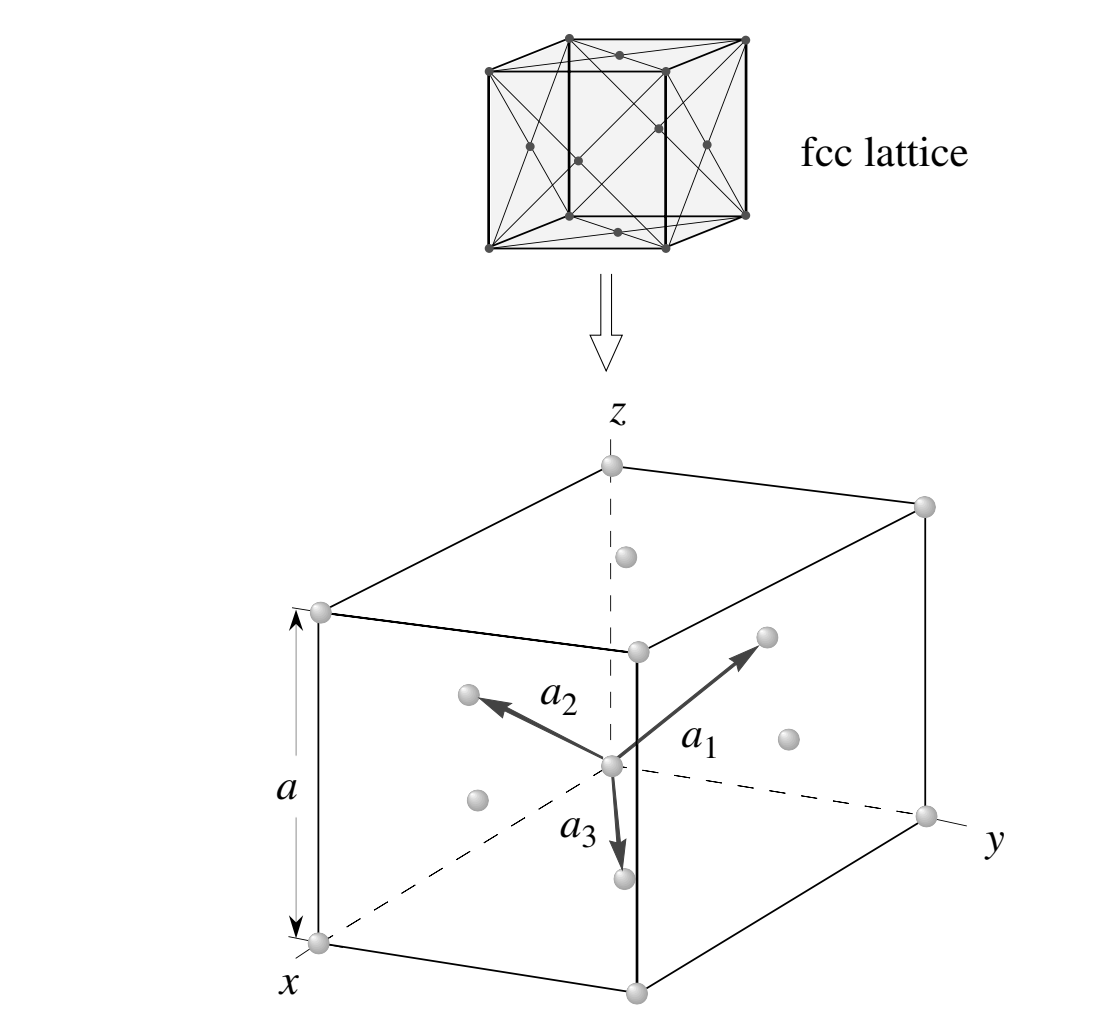
\includegraphics[width=\textwidth]{img/fcc.png}
		\\[0.5em]
		\refstepcounter{figure}
		\textbf{Figure~\thefigure.} Primitive vectors of the face-centered cubic (fcc) lattice.
		\label{fig:fcc_lattice}
	\end{minipage}
\end{center}

The face-centered cubic (fcc) Bravais lattice is another fundamental structure commonly found in semiconductors. It can be generated by starting with a simple cubic lattice and adding an extra lattice point at the center of each of the cube's faces.
A convenient and symmetric choice of primitive vectors for the fcc lattice is given by:
\begin{align*}
	\mathbf{a}_1 & = \frac{a}{2} (\hat{\mathbf{x}} + \hat{\mathbf{z}}) \\
	\mathbf{a}_2 & = \frac{a}{2} (\hat{\mathbf{y}} + \hat{\mathbf{z}}) \\
	\mathbf{a}_3 & = \frac{a}{2} (\hat{\mathbf{x}} + \hat{\mathbf{y}})
\end{align*}
Both the face-centered cubic and the body-centered cubic Bravais lattices play a crucial role in solid-state physics, as many materials crystallize in these arrangements, with atoms or ions located at each lattice point. Nearly all semiconductors relevant to electronics and optoelectronics adopt the fcc crystal structure.

\subsection{Basic Crystal Structures}
\subsubsection{Diamond and Zinc Blende Structures}
Most semiconductors relevant to electronics and optoelectronics are based on an underlying face-centered cubic (fcc) lattice. However, unlike simple fcc structures, they feature a basis consisting of two atoms. The positions of these two basis atoms are:
\begin{align*}
	(0, 0, 0) \quad \text{and} \quad \left( \frac{a}{4}, \frac{a}{4}, \frac{a}{4} \right)
\end{align*}

Because each of these atoms occupies its own fcc sublattice, the full crystal structure can be interpreted as two interpenetrating fcc lattices. One of these lattices is displaced from the other by a translation along the body diagonal direction:
\begin{align*}
	\frac{a}{4}(1, 1, 1)
\end{align*}
This type of arrangement gives rise to the well-known diamond and zinc blende structures, depending on the atomic species involved.

\subsubsection{Hexagonal Close-Packed (HCP) Structure}
The hexagonal close-packed (HCP) structure is another important crystal arrangement found in many materials, including some semiconductors. The HCP lattice can be visualized as a stacking of close-packed planes of atoms, with each plane being arranged in a hexagonal pattern.

The primitive vectors for the HCP lattice can be defined as follows:
\begin{align*}
	\mathbf{a}_1 & = \frac{a}{2} (\hat{\mathbf{x}} + \hat{\mathbf{y}})  \\
	\mathbf{a}_2 & = \frac{a}{2} (-\hat{\mathbf{x}} + \hat{\mathbf{y}}) \\
	\mathbf{a}_3 & = c \hat{\mathbf{z}}
\end{align*}
Here, \(c\) is the height of the hexagonal unit cell, and the relationship between \(a\) and \(c\) is determined by the packing efficiency of the structure.

The HCP structure is characterized by a coordination number of 12, meaning each atom is in contact with 12 others. This high coordination number contributes to the stability and strength of materials with an HCP crystal structure.

\subsubsection{Notation to Denote Planes and Points in a Lattice: Miller Indices}
A straightforward convention is used to describe lattice planes, directions, and points within a crystal. For lattice planes, the procedure is as follows:

\begin{enumerate}
	\item Define the coordinate axes (typically aligned with the primitive vectors).
	\item Determine where the plane intersects the $x$, $y$, and $z$ axes, using units of the lattice constants.
	\item Take the reciprocal of these intercepts and reduce the resulting values to the smallest set of integers.
\end{enumerate}

The resulting set of integers $(hkl)$ is used to denote a family of parallel lattice planes, referred to as a \textit{Miller index}. The notation $\{hkl\}$ indicates a family of crystallographically equivalent planes related by symmetry.

\section{Artificial Structures: Superlattices and Quantum Wells}
The electronic and optical characteristics of semiconductors can be significantly modified by forming heterostructures—combinations of different semiconductor materials. Advanced epitaxial growth techniques such as Molecular Beam Epitaxy (MBE) and Metal-Organic Chemical Vapor Deposition (MOCVD) enable precise control of the chemical composition at the monolayer scale (on the order of $\sim$3~\AA). These methods have been successfully used to grow a wide range of semiconductor materials, from those with zero bandgap like $\alpha$-Sn and HgCdTe, to wide bandgap compounds such as ZnSe and CdS.
Through heteroepitaxial growth, it is possible to fabricate layered structures with atomic-level precision, allowing intentional variation of the crystal’s periodicity along the growth direction. This leads to the creation of \textit{superlattices}, where two or more semiconductor materials—typically labeled A and B—are alternately deposited with respective thicknesses $d_A$ and $d_B$. The resulting periodicity in the growth direction is $d_A + d_B$. An example is the (GaAs)/(AlAs) superlattice. Remarkably, modern epitaxial techniques have achieved alternating layer thicknesses down to a single monolayer.
Although superlattices demonstrate the high precision of these growth methods, the most commonly used heterostructures in practical applications are \textit{quantum wells}. A quantum well consists of a thin layer of a lower bandgap semiconductor embedded between two layers of a higher bandgap material. These structures harness quantum mechanical effects, which are now essential in the operation of many electronic and optoelectronic devices.

\subsection{Surfaces: Ideal Versus Real}
The structural and electronic behavior of a crystal at its surface can differ significantly from that of the bulk. In the bulk, the crystal structure is determined by the minimization of internal chemical energy, with atoms adopting positions based on interactions with their nearest and next-nearest neighbors. However, at the surface, this balance is disrupted due to the abrupt reduction in the number of neighboring atoms.
As a result, the atomic arrangement that was energetically favorable within the bulk may no longer be optimal at the surface. To compensate, atoms at the surface often rearrange themselves into new configurations—known as \textit{surface reconstructions}—that lower the system’s total energy under the new boundary conditions.

\subsection{Interfaces}
Just like surfaces, interfaces play a critical role in the operation of semiconductor devices. In previous sections, we introduced heterostructures and superlattices, both of which inherently involve interfaces between different semiconductor materials. These interfaces are typically of very high quality, exhibiting minimal disruption in bonding—though defects such as dislocations can arise, particularly in strained-layer systems (which will be discussed later).
Despite the high crystalline quality, there is often a small degree of interface roughness—on the order of one to two monolayers. This can be attributed to factors such as suboptimal growth conditions or slight timing inaccuracies in the switching between different semiconductor elements during epitaxial growth. While the crystal lattice and its periodic structure are preserved across the interface, some degree of atomic disorder in the chemical composition can be present within the interfacial planes. This microscopic disorder can significantly impact the behavior of electronic and optoelectronic devices.
One of the most technologically significant interfaces is that between silicon and silicon dioxide (Si/SiO$_2$). The performance and scalability of nearly all modern electronic devices—including those that power the consumer electronics revolution—depend heavily on the exceptional quality of this interface. Interestingly, even though silicon and silicon dioxide differ substantially in both lattice constant and crystal structure, the interface is remarkably well-behaved. Typically, the transition region spans just a few monolayers and may include some degree of structural disorder or partial amorphization, leading to fluctuations in chemical composition that are important in determining device characteristics.

\section{Defects in Semiconductors}
In practical semiconductor materials, the presence of defects is inevitable. These imperfections may arise from thermodynamic factors or from unintentional contamination during the crystal growth process. Defects in crystalline semiconductors are generally classified into four categories:
\begin{enumerate}
	\item \textit{Point defects} — localized disruptions such as vacancies, interstitials, or substitutional atoms;
	\item \textit{Line defects} — also known as dislocations, which extend along one dimension;
	\item \textit{Planar defects} — including stacking faults or grain boundaries that span across planes;
	\item \textit{Volume defects} — such as precipitates or voids that affect larger regions of the material.
\end{enumerate}

These defects can significantly degrade the electrical and optical properties of semiconductor devices and are generally undesirable. Therefore, minimizing their occurrence is a key goal in semiconductor fabrication. In the following, we provide a brief introduction to the most relevant types of defects.

\subsection{Point Defects}
\begin{center}
	\begin{minipage}{0.9\textwidth}
		\centering
		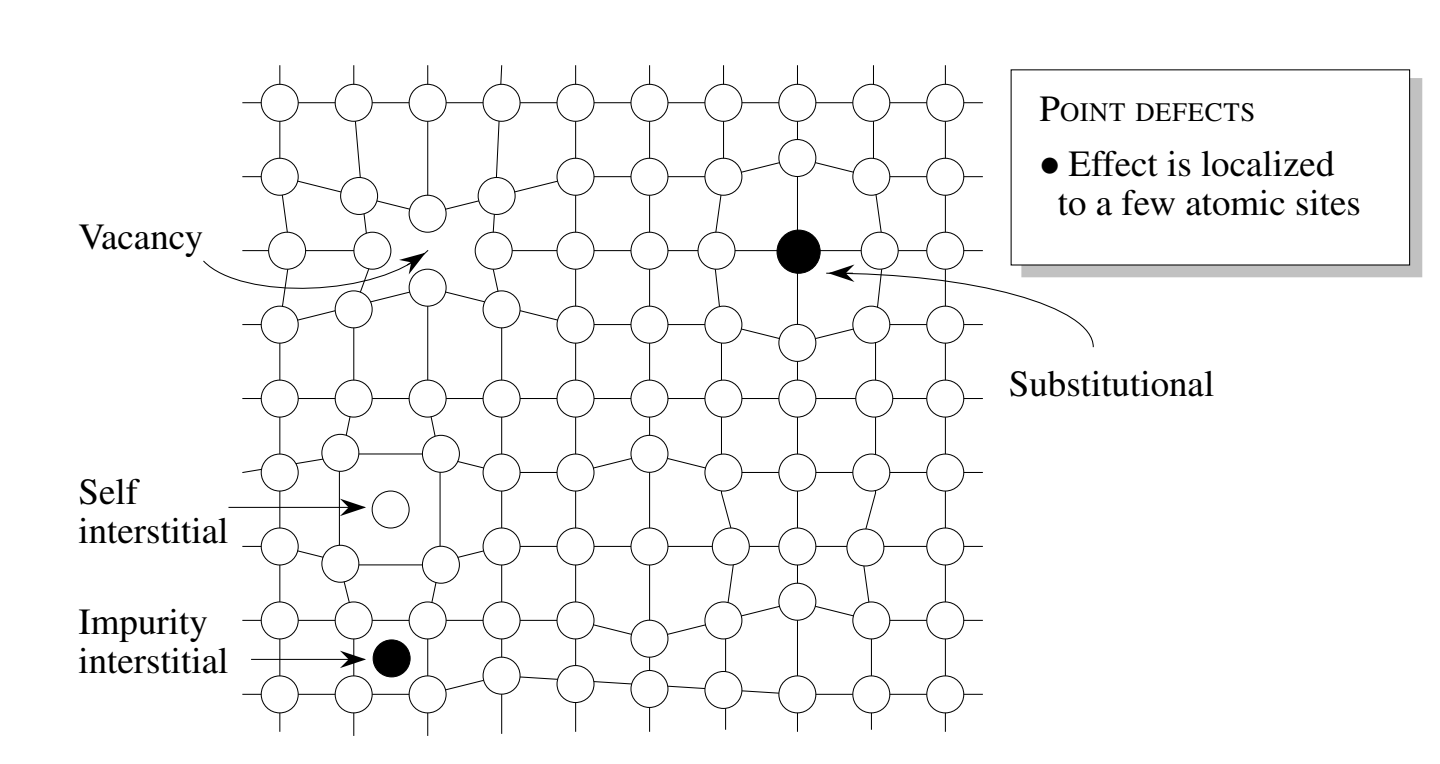
\includegraphics[width=\textwidth]{img/point_defects.png}
		\\[0.5em]
		\refstepcounter{figure}
		\textbf{Figure~\thefigure.} A schematic showing some important point defects in a crystal lattice.
		\label{fig:point_defects}
	\end{minipage}
\end{center}
Point defects are localized imperfections in a crystal lattice that disrupt the periodic structure only within one or a few unit cells. These types of defects are among the most fundamental and occur in all real crystalline materials. Their presence is governed by thermodynamic principles, and their equilibrium concentration can be estimated using the relation:
\begin{equation*}
	\frac{N_d}{N_\text{tot}} = k \exp\left( -\frac{E_d}{k_B T} \right)
\end{equation*}
where $N_d$ is the defect (e.g., vacancy) concentration, $N_\text{tot}$ is the total number of atomic sites in the crystal, $E_d$ is the defect formation energy, $k$ is a dimensionless constant typically ranging from 1 to 10 for semiconductors, $k_B$ is Boltzmann’s constant, and $T$ is the absolute temperature during crystal growth. For most semiconductors, the formation energy of a vacancy is typically on the order of an electronvolt.

A particularly significant point defect in compound semiconductors, such as GaAs, is the \textit{anti-site} defect. In this case, an atom from one sublattice—for example, a gallium (Ga) atom—occupies a site normally reserved for an arsenic (As) atom, resulting in a defect often denoted as Ga$_\text{As}$. These anti-site defects can act as deep traps or recombination centers, ultimately degrading the performance of electronic and optoelectronic devices.

\subsection{Line defects: Dislocations}
Unlike point defects, line defects—commonly referred to as dislocations—extend over many atomic sites and can be described by a line connecting the disrupted region. A typical example of a dislocation occurs when an extra half-plane of atoms is inserted or removed from the crystal, resulting in what is known as an \textit{edge dislocation}. Another form arises from shear deformation or crystal slip, where atomic planes shift and bonds are broken and reformed along a slip line.
Dislocations are particularly problematic in the growth of strained heterostructures, where lattice mismatch between different materials can induce mechanical stress. In optoelectronic devices, the presence of dislocations can lead to non-radiative recombination and significant degradation in device efficiency or even complete failure. For this reason, minimizing and controlling dislocation density is a critical aspect of high-quality semiconductor fabrication.
\begin{center}
	\begin{minipage}{0.6\textwidth}
		\centering
		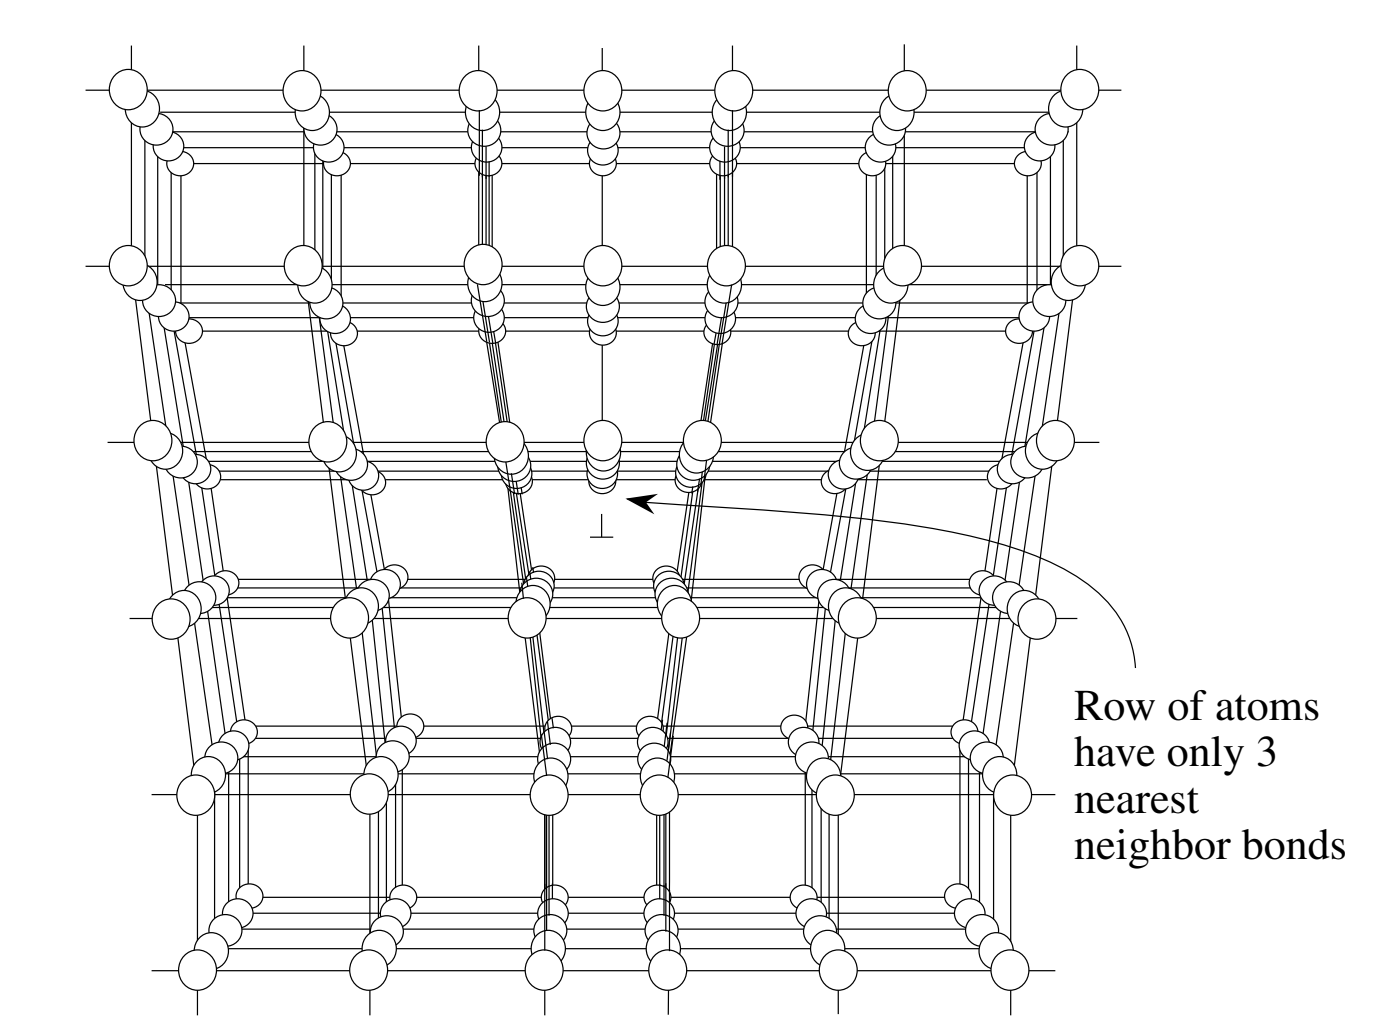
\includegraphics[width=\textwidth]{img/line_defects.png}
		\\[0.5em]
		\refstepcounter{figure}
		\textbf{Figure~\thefigure.} A schematic showing the presence of dislocation. The line defect is produced by adding an extra half plane of atoms. At the edge of the extra plane, the atoms have a missing bond.
	\end{minipage}
\end{center}


\section{Strained Heterostructures}
During epitaxial growth, the deposited layer (or overlayer) may possess a lattice constant that differs from that of the underlying substrate. When this occurs, the resulting structure is referred to as \textit{strained epitaxy}. This type of growth introduces strain in the crystal due to the lattice mismatch between the two materials. Strained epitaxy is a key area of research in modern crystal growth, as it enables the engineering of material properties through controlled strain, which can enhance the performance of electronic and optoelectronic devices.

\subsection{Coherent and Incoherent Structures}
Consider a scenario in which an epitaxial overlayer with lattice constant $a_L$ is deposited on a substrate with lattice constant $a_S$. The lattice mismatch between the two materials introduces strain, which can be quantified as:
\begin{equation*}
	\varepsilon = \frac{a_S - a_L}{a_L}
\end{equation*}
To understand the implications of this mismatch, imagine depositing a single monolayer of the overlayer onto the substrate. If the overlayer retains its natural lattice constant $a_L$, then after every $1/\varepsilon$ bonds, a discontinuity arises—either a missing or an extra bond—due to the misalignment. Since the interface is two-dimensional, these discontinuities form rows, giving rise to dislocations. Dislocations are energetically unfavorable because they leave some atoms at the interface improperly bonded, increasing the system’s total energy.
An alternative scenario is one where the overlayer adjusts its in-plane lattice constant to match that of the substrate. In this case, all interfacial atoms remain bonded, but the overlayer is placed under strain, storing strain energy in the crystal. As the layer grows thicker, this strain energy increases. Whether the system remains coherently strained or begins to introduce dislocations depends on a competition between the elastic strain energy and the energy cost of forming dislocations.
For small lattice mismatches (typically $\varepsilon < 0.1$), the overlayer can initially grow coherently, fully strained to the substrate. However, as thickness increases, it becomes energetically favorable for the system to relieve strain by forming dislocations. This transition is characterized by a so-called \textit{critical thickness}, $d_c$, which gives a rough estimate of the maximum thickness for coherent growth. A simplified expression for $d_c$ is:
\begin{equation*}
	d_c \sim \frac{a_S}{2|\varepsilon|}
\end{equation*}
In practice, the exact point at which dislocations begin to form depends on a range of factors, including growth temperature, surface morphology, and the kinetics of dislocation motion. Nonetheless, Equation~(1.14) provides a useful guideline for distinguishing between coherent and incoherent growth regimes for a given lattice mismatch.


\section{Strain Tensor in a lattice mismatched epitaxy}
To analyze how strain affects the electronic properties of semiconductors, one must first determine the strain tensor resulting from epitaxial growth. When an epitaxial layer is deposited on a substrate with a slightly different lattice constant, coherent strain can develop if the lattice mismatch is small and growth conditions are carefully controlled.
In such cases, the epitaxial layer undergoes \textit{pseudomorphic growth}, where the lattice constant of the layer in directions parallel to the interface is forced to match that of the substrate. As a result of this constraint, the perpendicular lattice constant adjusts according to the Poisson effect: if the layer is compressed in-plane, it expands out-of-plane, and if stretched in-plane, it contracts in the perpendicular direction.
For epitaxial growth that proceeds in a layer-by-layer fashion, the strain in the crystal is typically biaxial within the substrate plane and uniaxial in the perpendicular direction. The in-plane (biaxial) strain $\varepsilon_\parallel$ can be expressed in terms of the lattice constants of the substrate ($a_S$) and the epitaxial layer ($a_L$) as:
\begin{equation*}
	\varepsilon_\parallel = \frac{a_S - a_L}{a_L} = \frac{a_S}{a_L} - 1 = \varepsilon
\end{equation*}
This strain plays a fundamental role in modifying the band structure and other physical properties of the material.

\begin{figure}[h!]
    \centering
    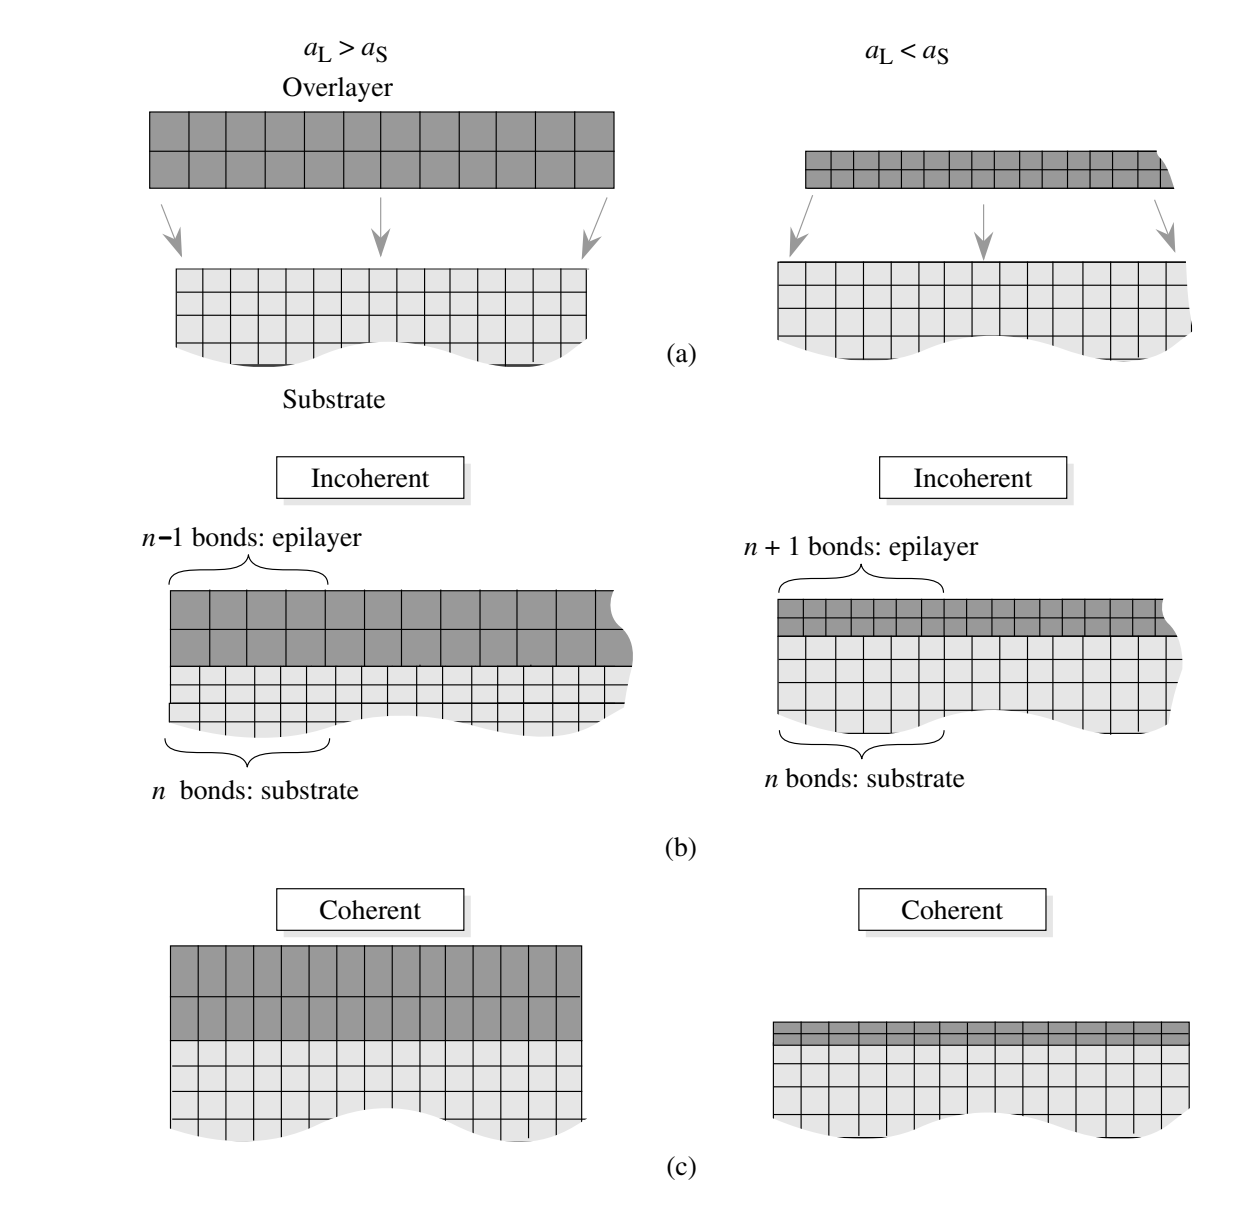
\includegraphics[width=0.8\textwidth]{img/coherentAndIncoherent.png}
    \caption{\small (a) Conceptual illustration of an overlayer with a lattice constant different from the substrate, placed without lattice distortion. (b) Dislocations form at the interface at positions where atomic bonding is disrupted due to lattice mismatch. (c) Coherent case where the overlayer is elastically strained to match the substrate, resulting in no dislocations at the interface.}
    \label{fig:coherent_incoherent}
\end{figure}
The strain tensor $\varepsilon$ in a crystal can be expressed in terms of the displacement gradient tensor $\mathbf{u}$, which describes how the atomic positions deviate from their equilibrium positions. The strain tensor is given by:
\begin{equation*}
 \varepsilon_{ij} = \frac{1}{2} \left( \frac{\partial u_i}{\partial x_j} + \frac{\partial u_j}{\partial x_i} \right)
\end{equation*}
where $i$ and $j$ denote the Cartesian coordinates (1, 2, 3 corresponding to $x$, $y$, and $z$ axes, respectively). The displacement gradient tensor $\mathbf{u}$ is defined as:
\begin{equation*}
 u_i = x_i - x_i^0
 \end{equation*}
 where $x_i$ is the current position of the atom and $x_i^0$ is its equilibrium position. The strain tensor captures how the crystal lattice deforms due to external forces or internal stresses, providing a complete description of the strain state in the material.
 
